\documentclass[12pt,letterpaper]{article}
\usepackage{graphicx,textcomp}
\usepackage{natbib}
\usepackage{setspace}
\usepackage{fullpage}
\usepackage{color}
\usepackage[reqno]{amsmath}
\usepackage{amsthm}
\usepackage{fancyvrb}
\usepackage{amssymb,enumerate}
\usepackage[all]{xy}
\usepackage{endnotes}
\usepackage{lscape}
\newtheorem{com}{Comment}
\usepackage{float}
\usepackage{hyperref}
\newtheorem{lem} {Lemma}
\newtheorem{prop}{Proposition}
\newtheorem{thm}{Theorem}
\newtheorem{defn}{Definition}
\newtheorem{cor}{Corollary}
\newtheorem{obs}{Observation}
\usepackage[compact]{titlesec}
\usepackage{dcolumn}
\usepackage{tikz}
\usetikzlibrary{arrows}
\usepackage{multirow}
\usepackage{xcolor}
\newcolumntype{.}{D{.}{.}{-1}}
\newcolumntype{d}[1]{D{.}{.}{#1}}
\definecolor{light-gray}{gray}{0.65}
\usepackage{url}
\usepackage{listings}
\usepackage{color}

\definecolor{codegreen}{rgb}{0,0.6,0}
\definecolor{codegray}{rgb}{0.5,0.5,0.5}
\definecolor{codepurple}{rgb}{0.58,0,0.82}
\definecolor{backcolour}{rgb}{0.95,0.95,0.92}

\lstdefinestyle{mystyle}{
	backgroundcolor=\color{backcolour},   
	commentstyle=\color{codegreen},
	keywordstyle=\color{magenta},
	numberstyle=\tiny\color{codegray},
	stringstyle=\color{codepurple},
	basicstyle=\footnotesize,
	breakatwhitespace=false,         
	breaklines=true,                 
	captionpos=b,                    
	keepspaces=true,                 
	numbers=left,                    
	numbersep=5pt,                  
	showspaces=false,                
	showstringspaces=false,
	showtabs=false,                  
	tabsize=2
}
\lstset{style=mystyle}
\newcommand{\Sref}[1]{Section~\ref{#1}}
\newtheorem{hyp}{Hypothesis}

\title{Problem Set 1}
\date{October 9, 2025}
\author{Applied Stats/Quant Methods 1\\
Shelly Veal-Upham\\
25337422}

\begin{document}
	\maketitle
	
	\vspace{.5cm}
	\section*{Question 1: Education}
	\subsection*{Question 1.1: Confidence Interval}

\lstinputlisting[language=R, firstline=35, lastline=67]{PS01_SVU.R}  
This process results in a 90 percent confidence interval of [94.13, 102.75]\\
\vspace{.5cm}
	\subsection*{Question 1.2: Hypothesis Testing}
	Before beginning, it is important to note our assumptions, namely
\begin{enumerate}
	\item That the data from the teacher's school is randomly sampled and therefore a good representation of the school population
	\item That the nation-wide student IQs are normally distributed about the mean, 100.
\end{enumerate}
\vspace{.5cm}
Now, for the actual process:
\begin{enumerate}
	\item First we establish the Null and Alternative Hypothesis:\\
	\lstinputlisting[language=R, firstline=71, lastline=72]{PS01_SVU.R}  
	\item Next, we derive the test statistic:\\ 
	\lstinputlisting[language=R, firstline=74, lastline=74]{PS01_SVU.R}  
	Which yields a value of -0.596.\\
	\item As the sample size (n) is less than 30, we will reference the t-distribution and use pt() to find the p-value for this test statistic:\\
	\lstinputlisting[language=R, firstline=79, lastline=79]{PS01_SVU.R}  
	Yielding p-value: 0.72
	\item Finally, interpreting this result by comparing it to our alpha level ($\alpha=0.05$.):\\
	Because 0.72 is greater than 0.05, we fail to reject the null hypothesis; we cannot say there is statistically significant evidence that this teacher's school's average IQ is above the national average school IQ.
\end{enumerate}

\newpage
	\section*{Question 2: Political Economy}
\noindent Researchers are curious about what affects the amount of money communities spend on addressing homelessness. The following variables constitute our data set about social welfare expenditures in the USA. \\
\vspace{.15cm}

\begin{tabular}{r|l}
	\texttt{State} &\emph{50 states in US} \\
	\texttt{Y} & \emph{per capita expenditure on shelters/housing assistance in state}\\
	\texttt{X1} &\emph{per capita personal income in state} \\
	\texttt{X2} &  \emph{Number of residents per 100,000 that are "financially insecure" in state}\\
	\texttt{X3} &  \emph{Number of people per thousand residing in urban areas in state} \\
	\texttt{Region} &  \emph{1=Northeast, 2= North Central, 3= South, 4=West} \\
\end{tabular}
\vspace{.25cm}
	\subsection*{Question 2.1: Correlations}
Using base R we can calculate correlations among the variables:
	\lstinputlisting[language=R, firstline=140, lastline=140]{PS01_SVU.R}  
This yields a matrix of correlations among the variables, which we can plot using package "corrplot":
	\lstinputlisting[language=R, firstline=148, lastline=148]{PS01_SVU.R}  
	
		\begin{figure}[h!]\centering
			\caption{\footnotesize Correlation Plot.}
			\label{fig:plot_1}
			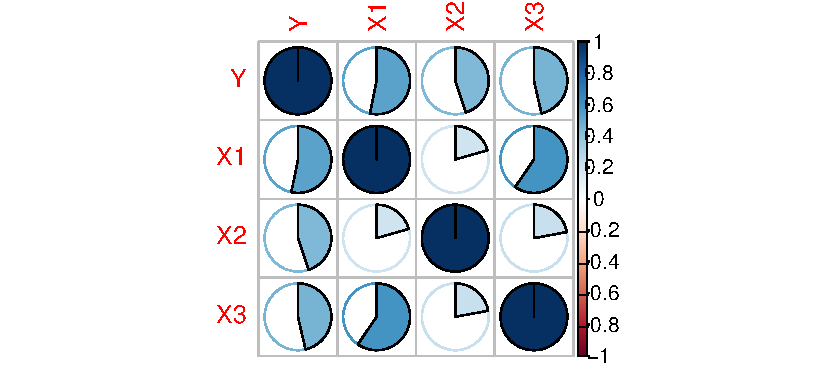
\includegraphics[width=.85\textwidth]{plot_2.1.pdf}
		\end{figure}
I chose method "pie" as this is most intuitive for me to visualize the different strengths of correlations between each variable pair.
\noindent As we can see, the strongest correlating input variable for output variable Y (Housing Expenditure) is X1 (Per Capita Personal Income), whereas the weakest correlating variable is X2 (Number of residentsper 100,000 that are "financially insecure" in state).
\noindent We can also see the strength of the relationships between each of the input variables, strongest being between X1 and X3.\\
	
\vspace{.5cm}
	\subsection*{Question 2.2: Y vs. Region}
Experimenting with the aggregate command in R, I created a plot of the total regional expenditures:
	\lstinputlisting[language=R, firstline=153, lastline=173]{PS01_SVU.R}  
	\begin{figure}[h!]\centering
		\caption{\footnotesize Total Regional Expenditures Plot.}
		\label{fig:plot_2.2.1}
		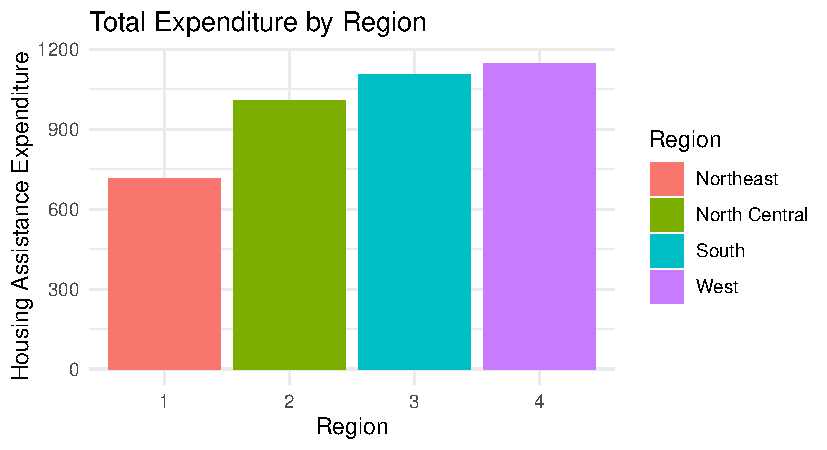
\includegraphics[width=.85\textwidth]{plot_2.2.1.pdf}
	\end{figure}
This plot is fine for viewing the data, but it doesn't help us compare the regions-- so we take the averages and compare those:
	\lstinputlisting[language=R, firstline=181, lastline=183]{PS01_SVU.R}  
	\begin{figure}[h!]\centering
		\caption{\footnotesize Average Regional Expenditures Plot.}
		\label{fig:plot_2.2.2}
		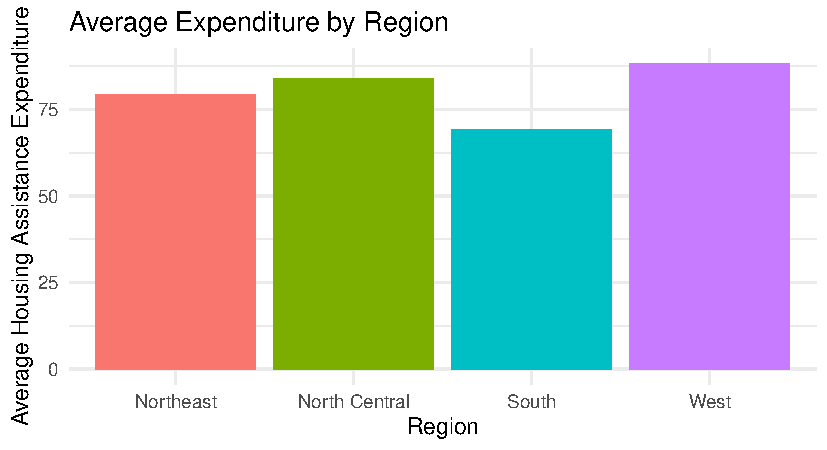
\includegraphics[width=.85\textwidth]{plot_2.2.2.pdf}
	\end{figure}
	
And finally, it's helpful to view the graph in descending order:
	\begin{figure}[h!]\centering
		\caption{\footnotesize Average Regional Expenditures Plot--Sorted.}
		\label{fig:plot_2.2.3}
		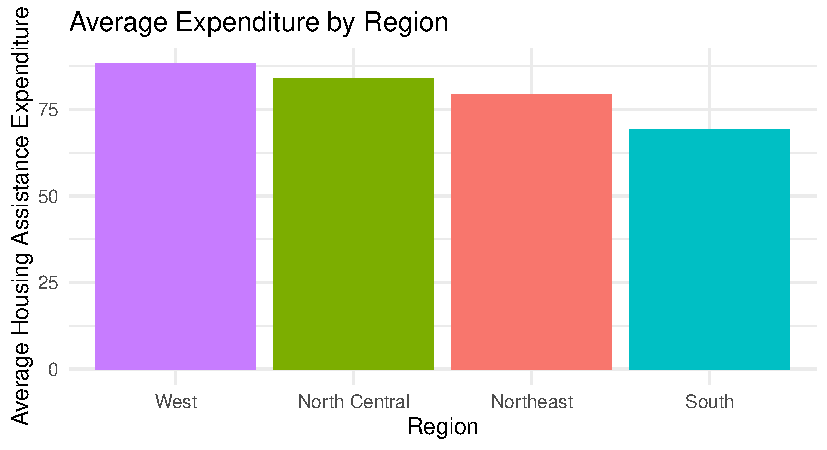
\includegraphics[width=.85\textwidth]{plot_2.2.3.pdf}
	\end{figure}

	\subsection*{Question 2.3: Y vs. X1}
	
\vspace{.25cm}
First, I took a general look at my data with a ggplot scatterplot:\\
	\lstinputlisting[language=R, firstline=227, lastline=239]{PS01_SVU.R}  
	\begin{figure}[h!]\centering
		\caption{\footnotesize Assistance vs Income Plot.}
		\label{fig:plot_2.3.1}
		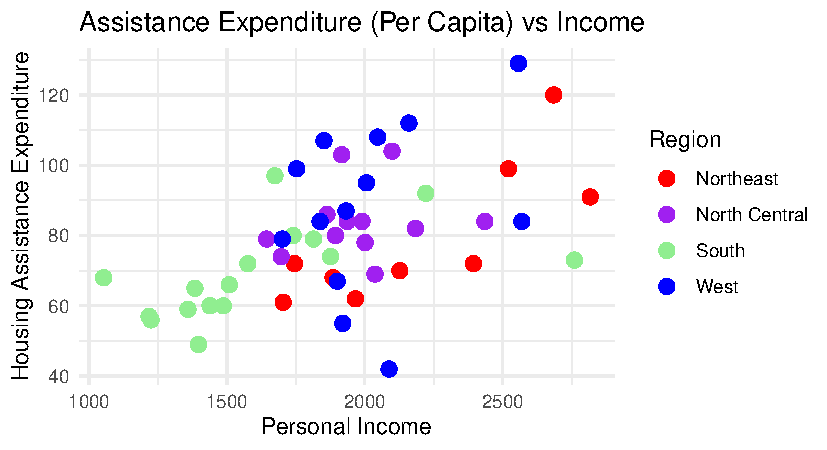
\includegraphics[width=.85\textwidth]{plot_2.3.1.pdf}
	\end{figure}

\newpage
Next, I added a regression line:\\
	\begin{figure}[h!]\centering
		\caption{\footnotesize AvI Plot with reg line.}
		\label{fig:plot_2.3.2}
		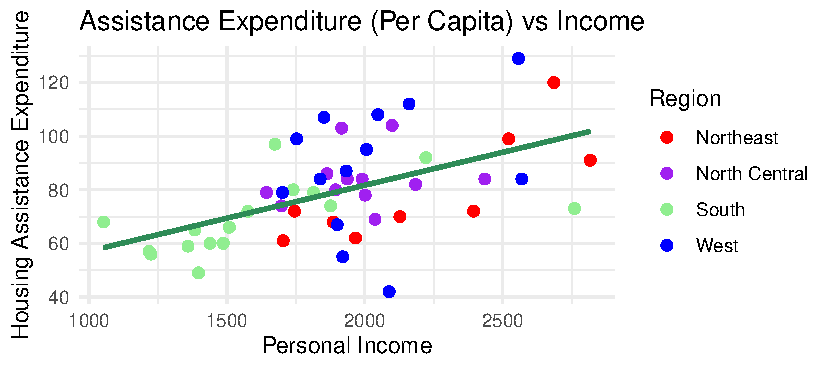
\includegraphics[width=.85\textwidth]{plot_2.3.2.pdf}
	\end{figure}

And finally added some fun shapes for the different regions:\\
\vspace{.15cm}
	\begin{figure}[h!]\centering
		\caption{\footnotesize AvI Plot with Shapes.}
		\label{fig:plot_2.3.3}
		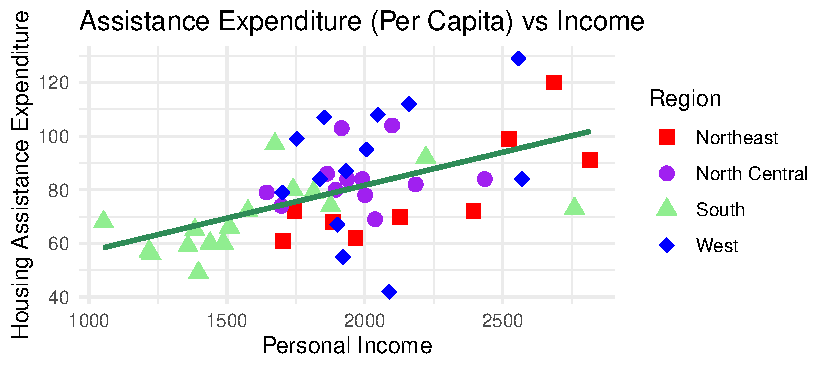
\includegraphics[width=.85\textwidth]{plot_2.3.3.pdf}
	\end{figure}
\vspace{0.15cm}

\newpage

We can see that there is a positive correlation between Y and X1 given that the regression line is positively sloped. This is in agreement with the pie chart we saw in the correlation plot above. All this is to say that there appears to be a reasonable positive correlation between Housing Assistance Expenditure and Personal Income by state.\\
The R code for my final plot (AvI Plot with Shapes) can be seen below:\\


	\lstinputlisting[language=R, firstline=260, lastline=288]{PS01_SVU.R}  
	
\end{document}
